\documentclass[letterpaper]{l3doc}

\hypersetup{urlcolor = teal, filecolor = violet}
\usepackage[mono = false]{libertine}
\usepackage{pdfpages,hologo,framed}
\hologoFontSetup{general = \sffamily}
\FrameSep = 0pt
\linespread{1.12}
\usepackage{indentfirst}
\setlength{\parindent}{2em}
\usepackage[os = mac]{menukeys}
\AddToHook{env/function/before}{\vspace{-.3\baselineskip}}
\AddToHook{env/syntax/after}{\vspace{-.2\baselineskip}}

\title
{
  \bfseries
  The \cls{litetable} Class: Colorful Timetable
  \thanks{\url{https://github.com/xiamyphys/litetable}}
}
\author
{
  Mingyu Xia \texttt{<\href{mailto:xiamyphys@gmail.com}{xiamyphys@gmail.com}>}
  \thanks{\href{https://github.com/ljguo1020}{Lijun Guo} developed modules for reading \meta{left} -> \meta{right} data structure and supporting low version \hologo {TeX} Live.}
}
\date{Version 3.1D, \today}

\begin{document}

\maketitle

\section{Introduction}

The \cls{litetable} class provides a design of timetable with colorful course boxes, which is based on the \cls{article} class, and conducted on \pkg{expl3} and \pkg{tikz}. It is compatible with \hologo{TeX}Live 2019 or later distributions, they all work fine for \hologo{pdfLaTeX} and \hologo{XeLaTeX} compilers. This is the Chinese manual for the \cls{litetable} class, manuals in \href{./litetable-cn.pdf}{Chinese} and \href{./litetable-hk.pdf}{Cantonese} versions are also provided\footnote{\href{https://qm.qq.com/q/RyssAhG4qy}{QQ Group: 760570712}}.

\section{Loading \cls{litetable} and generate the timetable frame}

Just like loading any class, write

\begin{framed}
  \begin{verbatim}
    \documentclass {litetable}
  \end{verbatim}
\end{framed}

One can load the \pkg{ctex} package and set the font to input the CJK characters, if necessary.

\begin{function}{\timelist,\weeklist}
  \begin{syntax}
    \cs{timelist} \oarg{rows} \marg{list}            \cs{timelist} \marg{list} \oarg{rows}
    \cs{weeklist} \oarg{default weeks} \marg{list}   \cs{weeklist} \marg{list} \oarg{default weeks}
  \end{syntax}

  The optional argument of the command \cs{timelist} can force the number of rows on the timetable, and that of the command \cs{weeklist} can set the default number of weeks and print it at every course box's southeast corner. Each mandatory argument of the two commands accepts an array that can add a time list to the left side of the timetable and add workdays with corresponding width ratios at the top of the timetable, respectively. The example for inputting the arrays is shown in Appendix \ref{mwe}.

  If the number of time arrays received by the command \cs{timelist} is greater than the forced number of rows, then the extra time sets are ignored, and it will return a warning. If one wants to add a series of numbers to the left side of the timetable without time, just leave the mandatory argument blank.
\end{function}

\begin{function}{\more}
  \begin{syntax}
    \cs{more} \marg{comment}
  \end{syntax}

  This command can add a comment at the southwest corner of the page.
\end{function}

\begin{function}{\maketable}
  \begin{syntax}
    \cs{maketable} \oarg{keyvals} \marg{title} \oarg{keyvals}
  \end{syntax}

  This command can create a blank timetable frame, and it should execute after commands \cs{timelist} and \cs{weeklist} in the \env{tikzpicture} environment with the option of \cmd{[remember picture, overaly]}. The optional argument accepts keys, it can set the background color of the timetable, and add the semester at the northeast corner of the page, the default value of the key \keys{\cmdmac~color} is \cmd{gray}. The mandatory argument can set the title.
\end{function}

\section{Add course boxes}

\begin{function}{\course}
  \begin{syntax}
    \cs{course} \oarg{keyvals} \marg{start number} \oarg{keyvals} \marg{end number} \oarg{keyvals}
  \end{syntax}
\end{function}

The \cs{course} command can add course boxes on the current workday, it should execute after command \cs{maketable} in the \env{tikzpicture} environment with the option of \cmd{[remember picture, overaly]}.

The optional argument accepts the following keys: \keys{\cmdmac~color} \keys{\cmdmac~subject} \keys{\cmdmac~location} \keys{\cmdmac~teacher} \keys{\cmdmac~weeks}. The default value of the key \keys{\cmdmac~color} is \cmd{teal}, and the default value of the key \keys{\cmdmac~weeks} is determined by the argument of the command \cs{weeklist}. The first and second mandatory arguments are the start and end numbers of the course, respectively.  The example of this command is shown in Appendix \ref{mwe}.

\begin{itemize}
  \item If the course box's height is only one unit, that is $\meta{start number} = \meta{end number}$, the values of keys \keys{\cmdmac~location} and \keys{\cmdmac~teacher} will print on the same line with a comma (,) separated, and the value of the key \keys{\cmdmac~weeks} will be hidden.
  \item If neither the key \keys{\cmdmac~location} nor the key \keys{\cmdmac~teacher} is assigned value, then the value of the key \keys{\cmdmac~subject} will print at the center of the course box.
  \item course boxes that are out of the timetable will not display, and it will return a warning.
\end{itemize}

\begin{function}{\newday}
  \begin{syntax}
    \cs{newday} \oarg{intergal value}
  \end{syntax}

  This command has an optional argument that can move the course boxes right \meta{intergal value} working days. The default value of the optional argument is \cmd{1} to move right \cmd{1} workday.
\end{function}

\clearpage\linespread{1.375}
\appendix

\section{Minimal Working Example}\label{mwe}

The following MWE could generate a timetable of 13 lines but only the top 12 lines have been marked with time, and there are 5 workdays at the top of the timetable, ratios between them are $4:5:4:6:5$. The default value of the key \keys{\cmdmac~weeks} will be set to \cmd{Weeks 1 - 16}. A comment and two course boxes are added.

\begin{framed}
  \begin{verbatim}
    \documentclass{litetable}

    \begin{document}

    \timelist [ 13 ]
      {
        08:05 -> 08:50, 08:55 -> 09:40, 10:00 -> 10:45, 10:50 -> 11:35,
        11:40 -> 12:25, 13:30 -> 14:15, 14:20 -> 15:05, 15:15 -> 16:00,
        16:05 -> 16:50, 18:30 -> 19:15, 19:20 -> 20:05, 20:10 -> 20:55
      }
    \weeklist [ Weeks 1 - 16 ]
      {
        Mon -> 4, Tue -> 5, Wed -> 4, Thu -> 6, Fri -> 5
      }
    \more { Author: Mingyu Xia \& Lijun Guo }

    \begin{tikzpicture} [ remember picture, overlay ]
      \maketable
      \course [ subject = Keep on {\TeX}ing ] {10} {11}
      \newday
      \course [ color = DarkSlateGray, subject = litetable,
                location = Hong Kong, teacher = M.Y. Xia
              ] {8} {8}
    \end{tikzpicture}

    \end{document}
  \end{verbatim}
\end{framed}

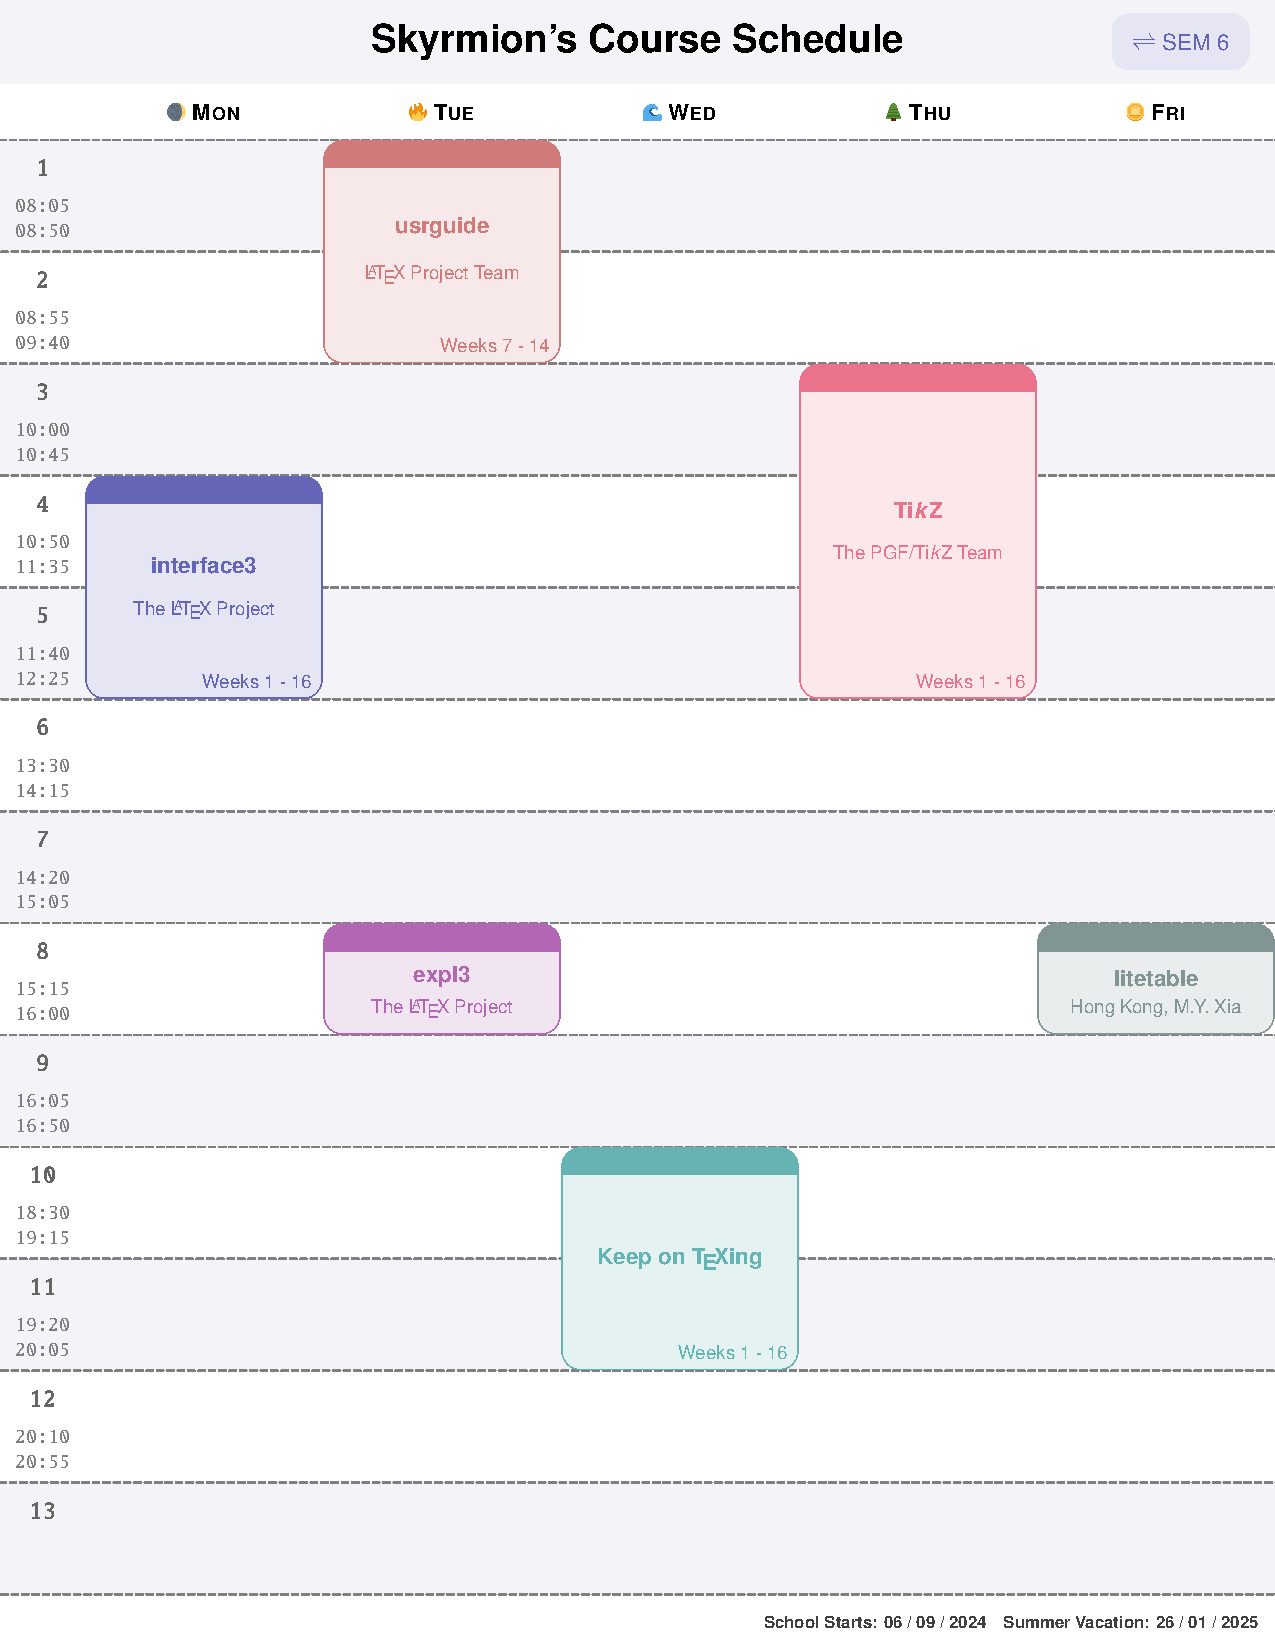
\includepdf[pages = 1]{litetable-demo.pdf}

\end{document}

% End of file litetable-en.tex
